% Provenance (never printed): cycle 2 "Questionner le monde de la matiere"
% (solid materials, observing and sorting) and cycle 3 theme 4 (local geology,
% rocks for building); see sources/book1/PROVENANCE.md. Book 1, grade 3, ch. 1.
\chapter{Cailloux, galets et sable}\label{ch:g3:stones-pebbles-sand}

Tom est en vacances au bord d'une \omterm{def:g1:landscapes-around-us:water}{rivière}. Sur la rive caillouteuse, là où
l'eau est peu profonde, il ramasse un \omterm{def:g3:stones-pebbles-sand:pebble}{galet}. Il est lisse et rond, presque
comme un œuf, et il tient dans sa main. La semaine dernière, en marchant
avec ses parents sur un sentier de \omterm{def:g1:landscapes-around-us:landform}{montagne}, tout en haut de la même
\omterm{def:g1:landscapes-around-us:landform}{vallée}, il a vu des cailloux de la même couleur au pied d'une pente
rocheuse --- mais ces cailloux étaient pointus, avec des arêtes et des
angles.

Comment un caillou pointu venu de la \omterm{def:g1:landscapes-around-us:landform}{montagne} est-il devenu un \omterm{def:g3:stones-pebbles-sand:pebble}{galet} lisse
et rond, en bas dans la \omterm{def:g1:landscapes-around-us:landform}{vallée}~? Pour le découvrir, commençons par la \omterm{def:g3:stones-pebbles-sand:rock}{roche}
elle-même.

\begin{omfigure}
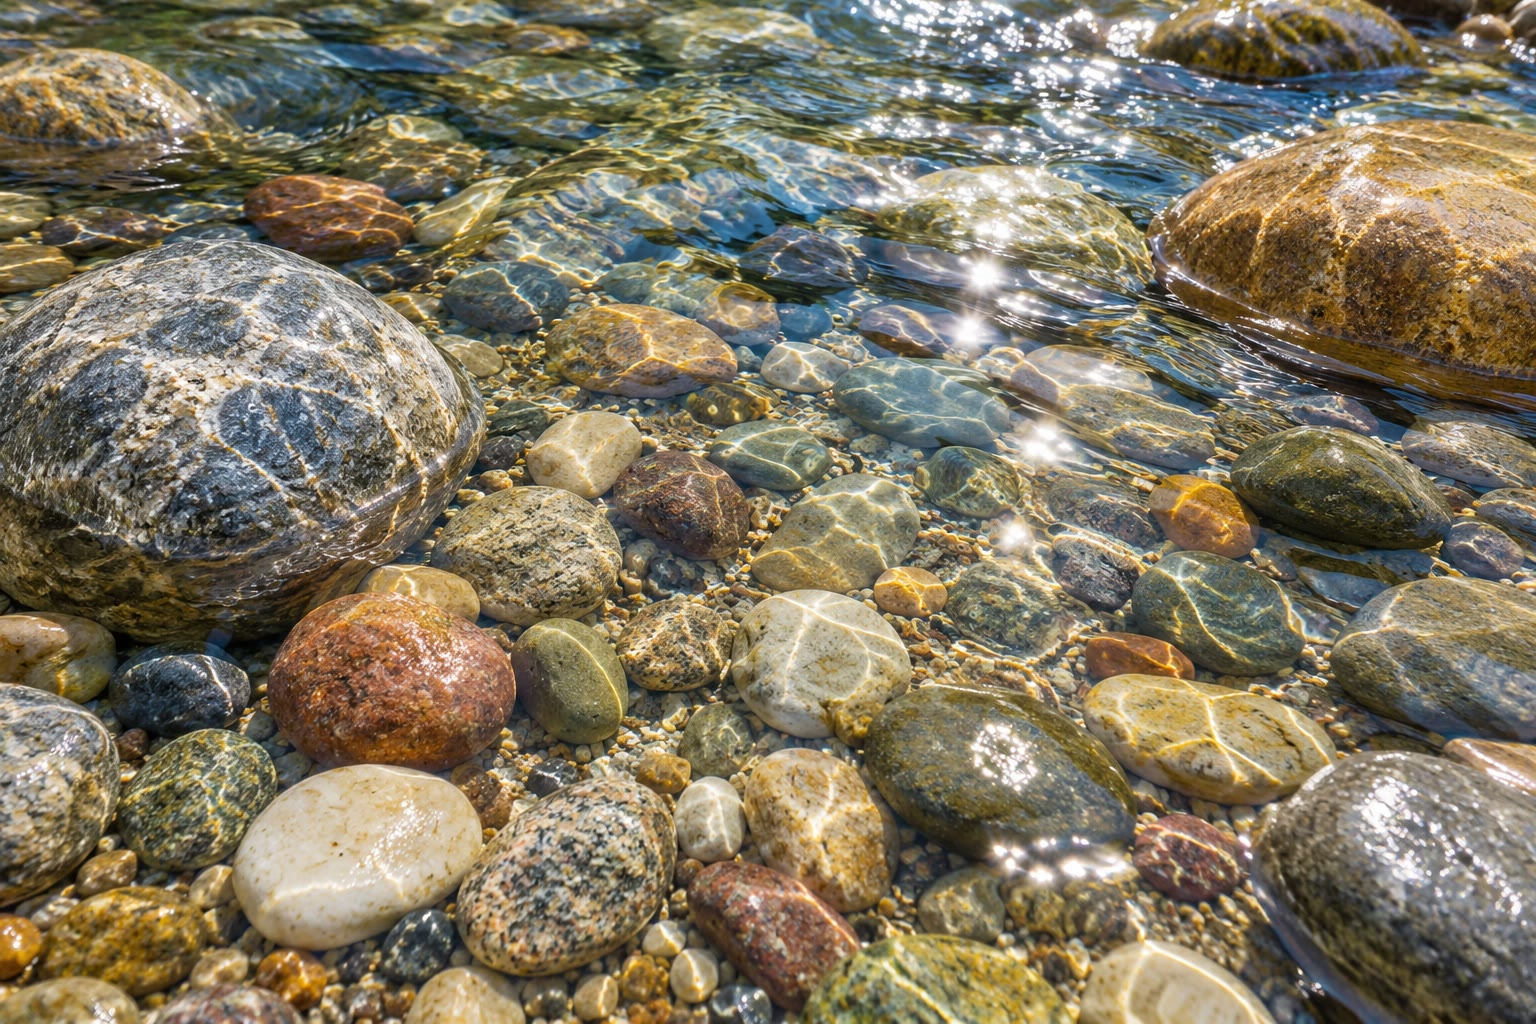
\includegraphics[width=0.62\linewidth]{images/book1/ai/g3-stream-pebbles.jpg}

{\small Des \omterm{def:g3:stones-pebbles-sand:pebble}{galets} ronds sous l'eau claire d'un ruisseau.}
\end{omfigure}

\begin{recall}
Dans un \omterm{def:g1:landscapes-around-us:landscape}{paysage}, il y a des \omterm{def:g1:landscapes-around-us:landform}{montagnes}, des \omterm{def:g1:landscapes-around-us:landform}{collines}, des \omterm{def:g1:landscapes-around-us:landform}{vallées} et des
\omterm{def:g1:landscapes-around-us:landform}{plaines}, et des \omterm{def:g1:landscapes-around-us:water}{rivières} qui coulent des terres hautes jusqu'à la \omterm{def:g2:water-on-earth:ocean}{mer}
(\cref{ch:g1:landscapes-around-us}). La couche du dessus, où poussent les
plantes, est le sol~: les livres de biologie racontent comment les êtres
vivants le fabriquent.
\end{recall}

\section{La roche~: le sol dur sous nos pieds}

Creuse un trou profond dans un jardin. Tu trouves d'abord une terre sombre
et meuble, pleine de racines. Plus bas, la terre devient plus claire et
plus caillouteuse. Et si tu pouvais creuser assez profond, tu arriverais
toujours à quelque chose de dur qu'une bêche ne peut pas couper~: la \omterm{def:g3:stones-pebbles-sand:rock}{roche}.

\begin{definition}[Roche et roche en place]\label{def:g3:stones-pebbles-sand:rock}
Une \emph{roche}\index{roche} est un matériau dur et naturel dont est faite
la Terre solide. La \emph{roche en place}\index{roche en place} est la roche
solide qui se trouve sous le sol partout sur les terres, et sous le \omterm{def:g3:stones-pebbles-sand:sand}{sable}
et la \omterm{def:g3:stones-pebbles-sand:sand}{boue} des fonds marins.
\end{definition}

Le plus souvent, la \omterm{def:g3:stones-pebbles-sand:rock}{roche en place} est cachée par le sol, l'herbe et les
arbres. Nous la voyons là où aucun sol ne la recouvre~: sur les flancs
raides des \omterm{def:g1:landscapes-around-us:landform}{montagnes}, dans les falaises au bord de la \omterm{def:g2:water-on-earth:ocean}{mer}, et le long des
routes taillées à travers une \omterm{def:g1:landscapes-around-us:landform}{colline}.

\begin{omfigure}
\begin{tikzpicture}[x=1cm, y=1cm, font=\small]
  % bedrock
  \fill[omLithGranite!60] (0,0) rectangle (11,2.2);
  \foreach \x/\y in {0.6/0.5, 1.8/1.4, 3.1/0.7, 4.4/1.6, 5.6/0.4, 6.9/1.2, 8.3/0.6, 9.6/1.5, 10.3/0.4}
    \draw[black!40, line width=0.4pt] (\x,\y) -- ++(0.5,0.25);
  % soil (thick on the left, missing on the steep right)
  \fill[brown!55] (0,2.2) -- (0,3.4) .. controls (2,3.5) and (4,3.4) .. (5.6,3.2) -- (6.4,2.9) -- (6.4,2.2) -- cycle;
  \fill[brown!30] (0,2.2) rectangle (6.4,2.65);
  % rock showing on the right: a hill side with no soil
  \fill[omLithGranite!60] (6.4,2.2) -- (6.4,2.9) -- (7.6,3.9) -- (8.8,4.3) -- (11,4.3) -- (11,2.2) -- cycle;
  \draw[black!60] (0,3.4) .. controls (2,3.5) and (4,3.4) .. (5.6,3.2) -- (6.4,2.9) -- (7.6,3.9) -- (8.8,4.3) -- (11,4.3);
  % grass and roots
  \foreach \x in {0.3,0.8,...,5.3}
    \draw[green!50!black, line width=0.6pt] (\x,{3.4-0.04*\x}) -- ++(0.05,0.18);
  \foreach \x in {1.2,3.4,4.9}
    \draw[brown!80!black, line width=0.5pt] (\x,3.3) -- ++(-0.1,-0.5) -- ++(0.15,-0.3);
  % labels
  \node[anchor=west] at (11.2,3.6) {roche visible};
  \node[anchor=west] at (11.2,3.2) {en surface};
  \draw[black!60] (11.15,3.4) -- (9.6,4.15);
  \node[anchor=east] at (-0.2,2.9) {sol};
  \draw[black!60] (-0.15,2.9) -- (0.6,2.9);
  \node[anchor=west] at (11.2,1.1) {roche en place};
  \draw[black!60] (11.15,1.1) -- (10.6,1.1);
\end{tikzpicture}

{\small Une coupe du terrain. Sous le sol, il y a toujours la \omterm{def:g3:stones-pebbles-sand:rock}{roche en
place}, solide. Sur le flanc raide de la \omterm{def:g1:landscapes-around-us:landform}{colline}, à droite, le sol manque et
la \omterm{def:g3:stones-pebbles-sand:rock}{roche} affleure à la surface.}
\label{fig:g3:stones-pebbles-sand:ground}
\end{omfigure}

\section{De la roche aux galets}

La \omterm{def:g3:stones-pebbles-sand:rock}{roche} est dure, mais elle ne dure pas éternellement. En hiver, l'eau
entre dans les fissures d'une \omterm{def:g3:stones-pebbles-sand:rock}{roche}, gèle, gonfle et écarte les fissures.
Les racines poussent aussi dans les fissures. Peu à peu, des morceaux se
détachent et tombent~: voilà d'où viennent les cailloux pointus au pied
des pentes de \omterm{def:g1:landscapes-around-us:landform}{montagne}.

Quand un caillou pointu tombe dans un torrent de \omterm{def:g1:landscapes-around-us:landform}{montagne}, l'eau le roule
sur le fond, le cogne contre d'autres cailloux et le traîne sur le \omterm{def:g3:stones-pebbles-sand:sand}{sable}.
Ses angles s'usent en premier. Plus il voyage loin, plus il devient rond et
lisse. Quand il arrive en bas de la \omterm{def:g1:landscapes-around-us:landform}{vallée}, il est devenu un \omterm{def:g3:stones-pebbles-sand:pebble}{galet}.

\begin{definition}[Galet et graviers]\label{def:g3:stones-pebbles-sand:pebble}
Un \emph{galet}\index{galet} est un petit morceau de \omterm{def:g3:stones-pebbles-sand:rock}{roche} arrondi et poli
par l'eau qui l'a roulé, dans une \omterm{def:g1:landscapes-around-us:water}{rivière} ou sur une plage. Les
\emph{graviers}\index{graviers} sont un amas de petites pierres et de
galets, dont les grains sont plus gros que des grains de \omterm{def:g3:stones-pebbles-sand:sand}{sable}.
\end{definition}

\begin{omfigure}
\begin{tikzpicture}[x=1cm, y=1cm, font=\small]
  \draw[ocBlue!70!black, line width=1.2pt, -{Stealth[length=3mm]}] (0,0) -- (12.2,0);
  \node[below, font=\scriptsize] at (6.1,-0.15) {le torrent emporte le caillou vers l'aval, un peu plus loin à chaque crue};
  \foreach \x/\shape/\t in {
     0.8/{(-0.55,-0.1) -- (-0.2,0.5) -- (0.35,0.55) -- (0.6,0.05) -- (0.3,-0.45) -- (-0.35,-0.5) -- cycle}/tombé de la roche,
     4.0/{(-0.5,-0.1) [rounded corners=4pt] -- (-0.2,0.45) -- (0.3,0.5) -- (0.55,0.05) -- (0.3,-0.4) -- (-0.35,-0.45) -- cycle}/angles usés,
     7.2/{(-0.45,-0.05) [rounded corners=8pt] -- (-0.15,0.42) -- (0.3,0.45) -- (0.5,0.05) -- (0.3,-0.35) -- (-0.3,-0.4) -- cycle}/plus rond et plus petit,
     10.4/{(0,0) ellipse (0.45 and 0.3)}/un galet lisse} {
    \begin{scope}[shift={(\x,1.1)}]
      \fill[omLithGranite!80, draw=black!70] \shape;
    \end{scope}
    \node[font=\scriptsize] at (\x,0.35) {\t};
  }
\end{tikzpicture}

{\small Le voyage d'un caillou dans une \omterm{def:g1:landscapes-around-us:water}{rivière}~: pointu quand il tombe de
la \omterm{def:g3:stones-pebbles-sand:rock}{roche}, rond et lisse après un long trajet vers l'aval.}
\label{fig:g3:stones-pebbles-sand:journey}
\end{omfigure}

\begin{remark}[Lire la forme d'un caillou]\label{rem:g3:stones-pebbles-sand:shape}
La forme d'un caillou raconte son histoire. Un caillou pointu n'a pas
voyagé loin de la \omterm{def:g3:stones-pebbles-sand:rock}{roche} dont il s'est détaché. Un \omterm{def:g3:stones-pebbles-sand:pebble}{galet} rond et lisse a
été longtemps roulé par l'eau, dans une \omterm{def:g1:landscapes-around-us:water}{rivière} ou par les vagues de la \omterm{def:g2:water-on-earth:ocean}{mer}.
\end{remark}

\section{Le sable et la boue}

Les cailloux et les \omterm{def:g3:stones-pebbles-sand:pebble}{galets} qui se cognent les uns contre les autres
perdent aussi de minuscules éclats. Au bout d'un temps très long, ces
minuscules éclats deviennent du \omterm{def:g3:stones-pebbles-sand:sand}{sable}. Regarde du \omterm{def:g3:stones-pebbles-sand:sand}{sable} à la loupe~:
chaque grain est un petit morceau de \omterm{def:g3:stones-pebbles-sand:rock}{roche}, ou de coquillage, souvent
arrondi lui aussi.

\begin{definition}[Sable et boue]\label{def:g3:stones-pebbles-sand:sand}
% ledger: usgs:wentworth
Le \emph{sable}\index{sable} est fait de grains libres de \omterm{def:g3:stones-pebbles-sand:rock}{roche} brisée,
plus petits que 2 millimètres~: nous voyons encore chaque grain. La
\emph{boue}\index{boue} est faite de grains si petits que nous ne pouvons
pas les voir un par un~; mouillée, elle est molle et collante.
\end{definition}

Les géologues trient les morceaux de \omterm{def:g3:stones-pebbles-sand:rock}{roche} brisée selon leur taille, du
plus gros au plus petit~: les blocs, les \omterm{def:g3:stones-pebbles-sand:pebble}{galets} et les \omterm{def:g3:stones-pebbles-sand:pebble}{graviers}, le \omterm{def:g3:stones-pebbles-sand:sand}{sable},
et la \omterm{def:g3:stones-pebbles-sand:sand}{boue}.

\begin{omfigure}
\begin{tikzpicture}[x=1mm, y=1mm, font=\small]
  % true size: 1 unit = 1 mm
  \draw[black!40] (0,-14) -- (150,-14);
  \foreach \x in {0,10,...,150} \draw[black!40] (\x,-14) -- (\x,-12.5);
  \foreach \x in {0,50,100,150} \node[font=\scriptsize, below] at (\x,-14.5) {\pgfmathparse{int(\x/10)}\pgfmathresult\,cm};
  % mud: too small
  \node[font=\scriptsize, align=center] at (6,14) {boue};
  \fill[brown!60] (6,0) circle (0.05);
  \node[font=\scriptsize, align=center] at (6,4.5) {grains trop\\petits pour être vus};
  % sand grains: up to 2 mm
  \node[font=\scriptsize] at (28,14) {sable};
  \foreach \x/\r in {22/0.3, 25/0.5, 28/0.75, 32/1.0}
    \fill[yellow!60!brown, draw=black!50, line width=0.2pt] (\x,0) circle (\r);
  \node[font=\scriptsize, align=center] at (28,5) {plus petits que\\2 millimètres};
  % gravel and pebbles
  \node[font=\scriptsize] at (78,22) {graviers et galets};
  \fill[omLithGranite!80, draw=black!60] (52,0) ellipse (2 and 1.5);
  \fill[black!25, draw=black!60] (62,0) ellipse (4 and 3);
  \fill[omLithGranite!80, draw=black!60] (78,0) ellipse (8 and 6);
  \fill[black!30, draw=black!60] (104,0) ellipse (15 and 10);
  % boulder: off scale
  \node[font=\scriptsize] at (138,22) {bloc};
  \fill[black!20, draw=black!60] (128,-10) .. controls (127,8) and (135,16) .. (142,15) .. controls (150,14) and (152,4) .. (149,-10) -- cycle;
  \node[font=\scriptsize, align=center, fill=white, fill opacity=0.7, text opacity=1, inner sep=1pt] at (139,4) {dessiné bien\\trop petit};
\end{tikzpicture}

{\small Les grains de \omterm{def:g3:stones-pebbles-sand:rock}{roche} brisée, du plus petit au plus gros. La \omterm{def:g3:stones-pebbles-sand:sand}{boue}, le
\omterm{def:g3:stones-pebbles-sand:sand}{sable}, les \omterm{def:g3:stones-pebbles-sand:pebble}{graviers} et les \omterm{def:g3:stones-pebbles-sand:pebble}{galets} sont dessinés à leur taille réelle~:
compare avec une règle. Un bloc peut être aussi gros qu'une chaise, ou
qu'une maison.}
\label{fig:g3:stones-pebbles-sand:sizes}
\end{omfigure}

\begin{omfigure}
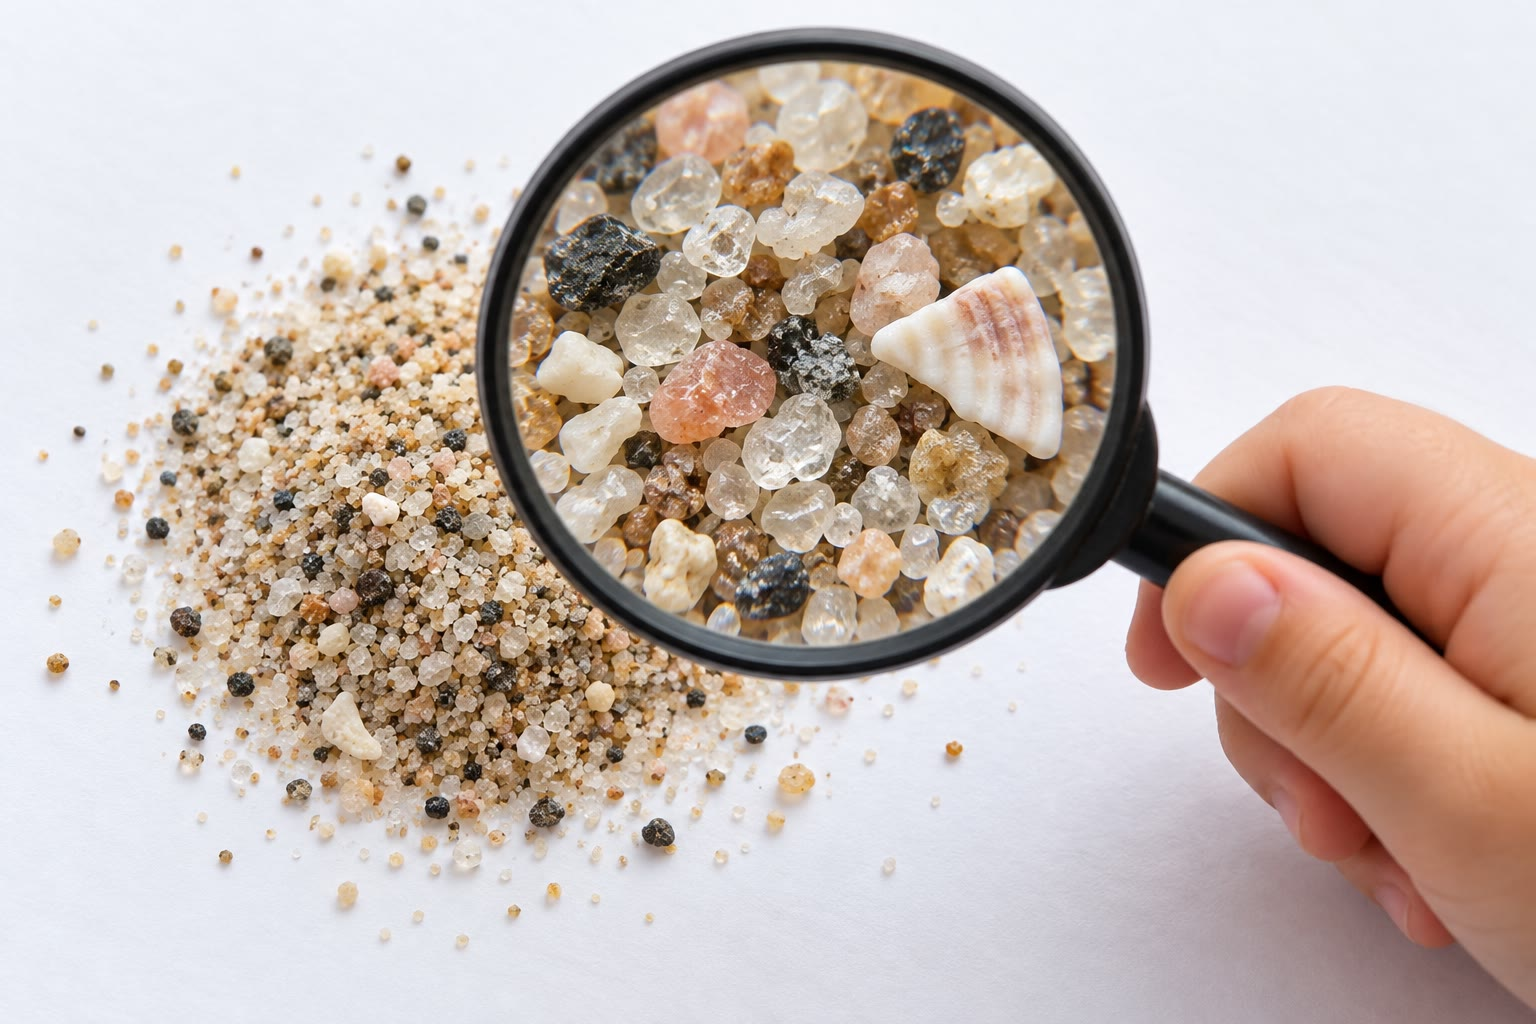
\includegraphics[width=0.55\linewidth]{images/book1/ai/g3-sand-magnifier.jpg}

{\small Du \omterm{def:g3:stones-pebbles-sand:sand}{sable} de plage vu à la loupe~: de minuscules grains de \omterm{def:g3:stones-pebbles-sand:rock}{roche} et
des morceaux de coquillages.}
\end{omfigure}

\begin{method}[Trier la roche brisée selon la taille]\label{met:g3:stones-pebbles-sand:sort}
Pour nommer un morceau de \omterm{def:g3:stones-pebbles-sand:rock}{roche} brisée, regarde sa taille~:
\begin{enumerate}
  \item si tu ne vois pas les grains, même de près, c'est de la \omterm{def:g3:stones-pebbles-sand:sand}{boue}~;
  \item si tu vois chaque grain, mais que chacun est plus petit que
        2 millimètres (l'épaisseur d'une pièce de monnaie), c'est du \omterm{def:g3:stones-pebbles-sand:sand}{sable}~;
  \item si les morceaux sont plus gros, mais que tu peux en tenir un dans
        ta main, ce sont des \omterm{def:g3:stones-pebbles-sand:pebble}{graviers} et des \omterm{def:g3:stones-pebbles-sand:pebble}{galets}~;
  \item si un morceau est trop lourd pour être soulevé, c'est un bloc.
\end{enumerate}
\end{method}

\begin{example}[Où trouve-t-on chaque taille~?]\label{ex:g3:stones-pebbles-sand:where}
Une eau rapide peut emporter de gros cailloux~; une eau lente les dépose
et n'emporte que de petits grains. C'est pourquoi les blocs et les
cailloux pointus se trouvent dans les torrents de \omterm{def:g1:landscapes-around-us:landform}{montagne} en pente
raide~; les \omterm{def:g3:stones-pebbles-sand:pebble}{galets} et les \omterm{def:g3:stones-pebbles-sand:pebble}{graviers} sur les rives de la \omterm{def:g1:landscapes-around-us:water}{rivière} dans la
\omterm{def:g1:landscapes-around-us:landform}{vallée}~; le \omterm{def:g3:stones-pebbles-sand:sand}{sable} s'accumule sur les plages et dans les courbes calmes de
la \omterm{def:g1:landscapes-around-us:water}{rivière}~; et la \omterm{def:g3:stones-pebbles-sand:sand}{boue} se dépose là où l'eau est presque immobile, dans
les mares, les \omterm{def:g1:landscapes-around-us:water}{lacs} et à l'embouchure des \omterm{def:g1:landscapes-around-us:water}{rivières}.
\end{example}

\section{Les roches dures et les roches tendres}

Toutes les \omterm{def:g3:stones-pebbles-sand:rock}{roches} ne sont pas aussi dures. Certaines, comme le granite,
sont si dures qu'elles rayent le verre et durent des milliers d'années
dans un mur. D'autres s'effritent dans la main, comme la craie, qui laisse
une trace blanche sur un tableau. Certaines \omterm{def:g3:stones-pebbles-sand:rock}{roches} sont faites de grains
que nous pouvons voir~; d'autres sont lisses et semblent partout pareilles.

\begin{example}[Trois roches comparées]\label{ex:g3:stones-pebbles-sand:three}
Le \emph{granite} est tacheté de grains roses, blancs et noirs, et il est
très dur. Le \emph{grès} est fait de grains de \omterm{def:g3:stones-pebbles-sand:sand}{sable} collés ensemble~;
frotté avec un doigt, il laisse parfois partir quelques grains. La
\emph{craie} est blanche, tendre et poudreuse. Tu apprendras dans une
année suivante comment chacune de ces \omterm{def:g3:stones-pebbles-sand:rock}{roches} s'est formée.
\end{example}

\begin{omfigure}
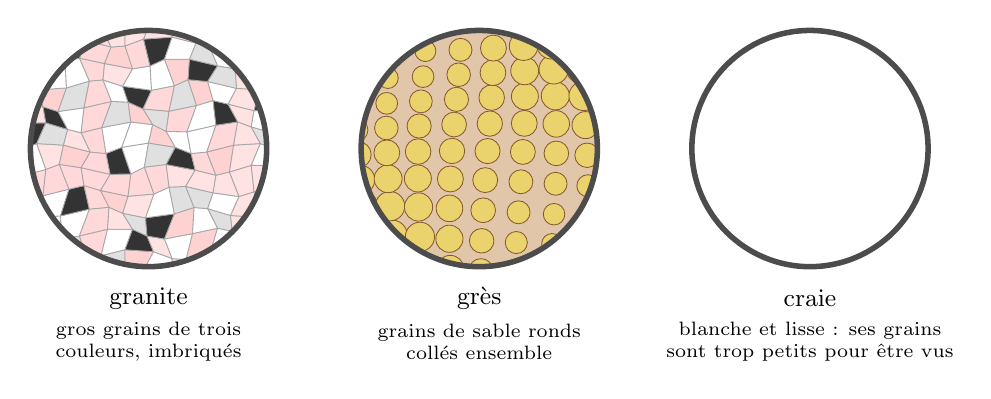
\begin{tikzpicture}[font=\small]
  % three stones seen through a magnifying glass (drawn, not to scale)
  % granite: interlocking grains of three colours
  \begin{scope}
    \clip (0,0) circle (1.5);
    % a jittered lattice: the cells tile the disk with no gap, like the
    % interlocking crystals of granite
    \foreach \i in {-6,...,5} \foreach \j in {-6,...,5} {
      \pgfmathtruncatemacro{\c}{mod(abs(37*\i+17*\j+\i*\j),7)}
      \ifcase\c \def\col{pink!70}\or\def\col{pink!45}\or\def\col{white}\or
        \def\col{black!12}\or\def\col{white}\or\def\col{black!80}\else\def\col{pink!60}\fi
      \fill[\col, draw=black!35, line width=0.3pt]
        ({0.27*\i+0.07*sin(90*\i+131*\j)},{0.27*\j+0.07*cos(77*\i+61*\j)}) --
        ({0.27*(\i+1)+0.07*sin(90*(\i+1)+131*\j)},{0.27*\j+0.07*cos(77*(\i+1)+61*\j)}) --
        ({0.27*(\i+1)+0.07*sin(90*(\i+1)+131*(\j+1))},{0.27*(\j+1)+0.07*cos(77*(\i+1)+61*(\j+1))}) --
        ({0.27*\i+0.07*sin(90*\i+131*(\j+1))},{0.27*(\j+1)+0.07*cos(77*\i+61*(\j+1))}) -- cycle;
    }
  \end{scope}
  \draw[black!70, line width=2pt] (0,0) circle (1.5);
  \node at (0,-1.9) {granite};
  \node[font=\scriptsize, align=center] at (0,-2.45) {gros grains de trois\\couleurs, imbriqués};
  % sandstone: rounded grains touching
  \begin{scope}[xshift=4.2cm]
    \clip (0,0) circle (1.5);
    \fill[brown!45] (-1.6,-1.6) rectangle (1.6,1.6);
    \foreach \x in {-1.5,-1.1,...,1.6} \foreach \y in {-1.5,-1.15,...,1.6}
      \fill[yellow!50!brown!70, draw=brown!70!black, line width=0.3pt]
        ({\x+0.08*sin(97*\x+61*\y)},{\y+0.07*cos(53*\x-89*\y)}) circle ({0.16+0.03*sin(71*\x*\y)});
  \end{scope}
  \draw[black!70, line width=2pt] (4.2,0) circle (1.5);
  \node at (4.2,-1.9) {grès};
  \node[font=\scriptsize, align=center] at (4.2,-2.45) {grains de sable ronds\\collés ensemble};
  % chalk: smooth, no grains to see
  \begin{scope}[xshift=8.4cm]
    \fill[white] (0,0) circle (1.5);
  \end{scope}
  \draw[black!70, line width=2pt] (8.4,0) circle (1.5);
  \node at (8.4,-1.9) {craie};
  \node[font=\scriptsize, align=center] at (8.4,-2.45) {blanche et lisse~: ses grains\\sont trop petits pour être vus};
\end{tikzpicture}

{\small Trois \omterm{def:g3:stones-pebbles-sand:rock}{roches} vues à la loupe (dessin). On voit les grains du
granite et du grès~; la craie paraît partout pareille.}
\label{fig:g3:stones-pebbles-sand:magnified}
\end{omfigure}

\begin{method}[Observer un caillou de près]\label{met:g3:stones-pebbles-sand:look}
Pour décrire un caillou, regarde-le et touche-le, sans le casser~:
\begin{enumerate}
  \item sa couleur, ou ses couleurs~;
  \item sa forme~: pointue avec des angles, ou ronde et lisse~;
  \item ses grains~: peux-tu les voir~? sont-ils tous pareils, ou de
        plusieurs couleurs~?
  \item au toucher~: est-il dur, ou assez tendre pour laisser une trace
        sur le papier~?
\end{enumerate}
Note ce que tu vois dans un tableau, une ligne pour chaque caillou.
\end{method}

\begin{example}[Un tableau de trois cailloux]\label{ex:g3:stones-pebbles-sand:table}
Mia décrit trois cailloux d'une boîte de l'école.
\begin{center}\small
\begin{tabular}{llll}
\hline
Caillou & Couleur & Forme & Grains \\
\hline
A & rose, blanc et noir & rond & gros, trois couleurs \\
B & brun-jaune & pointu & petits, tous pareils \\
C & blanc & pointu & invisibles \\
\hline
\end{tabular}
\end{center}
Le caillou C laisse aussi une trace blanche sur le papier. D'après
l'exemple ci-dessus, le caillou A ressemble à du granite, le caillou B à du
grès et le caillou C à de la craie. Le caillou A est rond~: l'eau l'a roulé
longtemps.
\end{example}

\section{Les pierres avec lesquelles nous construisons}

Depuis des milliers d'années, les gens construisent avec la \omterm{def:g3:stones-pebbles-sand:rock}{roche} qui les
entoure. Dans les vieux villages d'une région, les murs ont souvent tous
la même couleur, parce qu'ils ont été bâtis avec la pierre de la \omterm{def:g1:landscapes-around-us:landform}{colline}
la plus proche.

\begin{definition}[Pierre de construction]\label{def:g3:stones-pebbles-sand:building-stone}
Une \emph{pierre de construction}\index{pierre de construction} est une
\omterm{def:g3:stones-pebbles-sand:rock}{roche} que l'on taille ou que l'on façonne pour bâtir des murs, des toits,
des marches, des ponts ou des pavés.
\end{definition}

Chaque \omterm{def:g3:stones-pebbles-sand:rock}{roche} est bonne pour quelque chose. Le granite, très dur, donne des
murs, des marches et des bordures de trottoir qui durent des siècles.
Certaines \omterm{def:g3:stones-pebbles-sand:rock}{roches}, comme l'ardoise, se fendent en feuilles minces et
plates~: posées les unes sur les autres, elles font des toits qui
arrêtent la pluie. Le grès et le calcaire sont assez tendres pour être
taillés en blocs réguliers.

\begin{omfigure}
\begin{minipage}[b]{0.49\linewidth}\centering
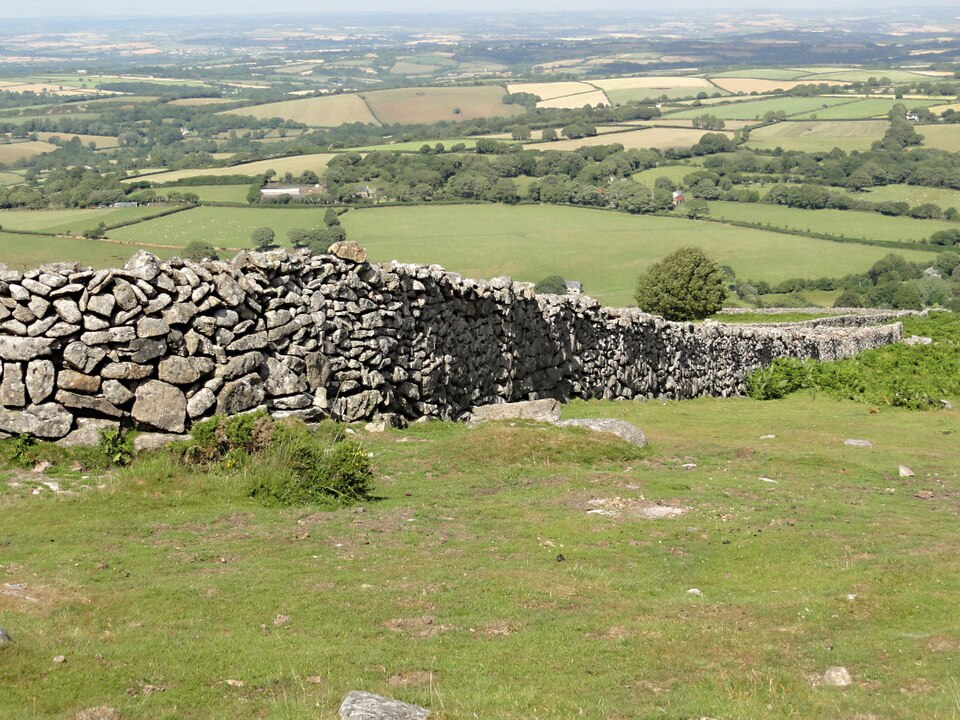
\includegraphics[width=\linewidth]{images/book1/g3-granite-wall.jpg}

{\small Un mur de blocs de granite, bâti sans mortier. Photographie~: Tony
Atkin, Geograph (CC BY-SA 2.0).}
\end{minipage}\hfill
\begin{minipage}[b]{0.49\linewidth}\centering
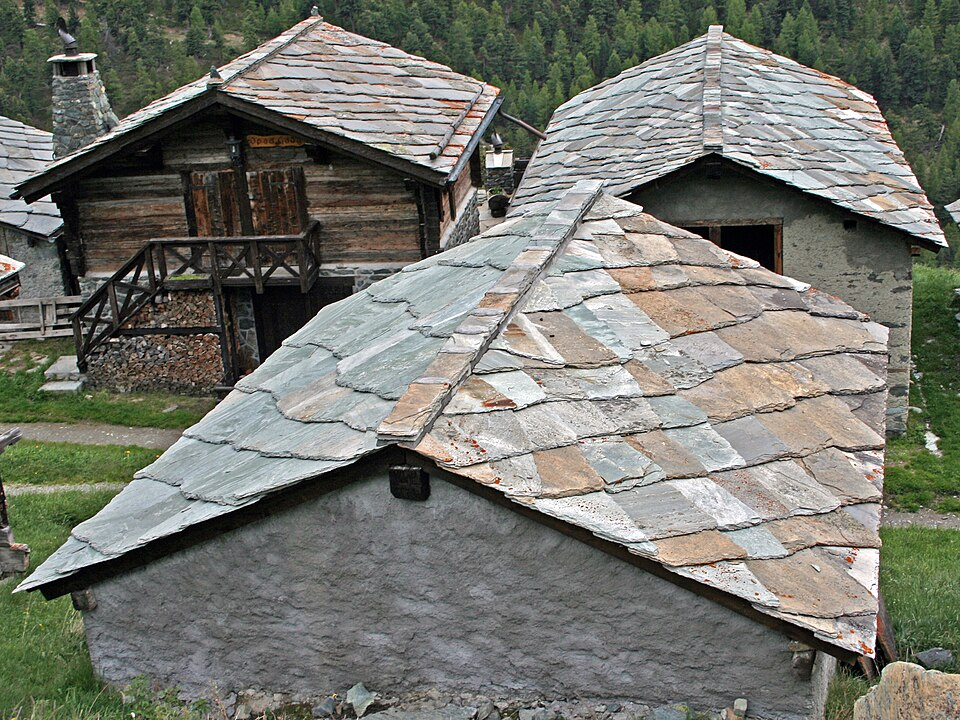
\includegraphics[width=\linewidth]{images/book1/g3-slate-roof.jpg}

{\small Des toits de dalles de pierre minces et plates dans un village de
\omterm{def:g1:landscapes-around-us:landform}{montagne} en Suisse. Photographie~: Michael C. Rygel (CC BY-SA 3.0).}
\end{minipage}
\end{omfigure}

\begin{omfigure}
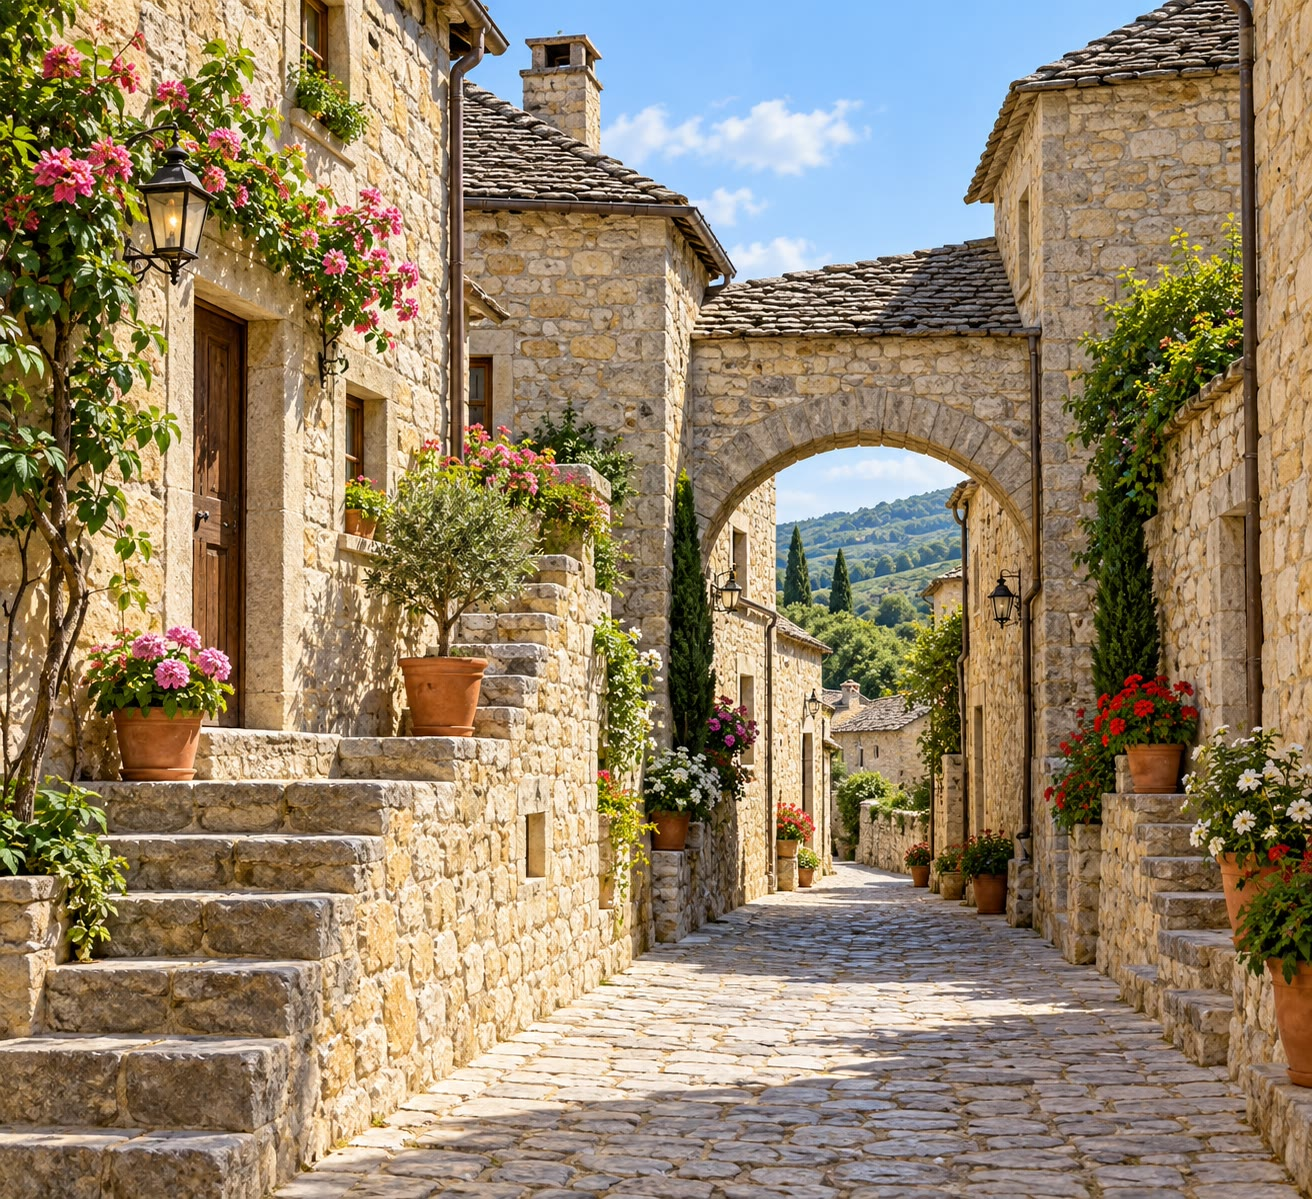
\includegraphics[width=0.6\linewidth]{images/book1/ai/g3-stone-village.jpg}

{\small Un vieux village entièrement bâti avec la pierre de la \omterm{def:g1:landscapes-around-us:landform}{colline} voisine.}
\end{omfigure}

Aujourd'hui, nous construisons aussi avec des briques, du béton et du
verre. Mais une brique est faite d'argile cuite, le béton est fait de
\omterm{def:g3:stones-pebbles-sand:sand}{sable}, de \omterm{def:g3:stones-pebbles-sand:pebble}{graviers} et de ciment, et le verre est fabriqué à partir de
\omterm{def:g3:stones-pebbles-sand:sand}{sable}~: tous viennent eux aussi des \omterm{def:g3:stones-pebbles-sand:rock}{roches} de la Terre.

\section{Exercices}

\begin{exercise}[$\star$]\label{exo:g3:stones-pebbles-sand:1}
Qu'est-ce que la \omterm{def:g3:stones-pebbles-sand:rock}{roche en place}~? Où peut-on la voir sans creuser~?
\end{exercise}

\begin{exercise}[$\star$]\label{exo:g3:stones-pebbles-sand:2}
Range par ordre de taille, du plus petit au plus gros~: \omterm{def:g3:stones-pebbles-sand:pebble}{galet}, \omterm{def:g3:stones-pebbles-sand:sand}{boue}, bloc,
\omterm{def:g3:stones-pebbles-sand:sand}{sable}.
\end{exercise}

\begin{exercise}[$\star$]\label{exo:g3:stones-pebbles-sand:3}
Un grain mesure 1 millimètre. Est-ce du \omterm{def:g3:stones-pebbles-sand:sand}{sable} ou du gravier~? Un autre
grain mesure 3 millimètres~: \omterm{def:g3:stones-pebbles-sand:sand}{sable} ou gravier~?
\end{exercise}

\begin{exercise}[$\star$]\label{exo:g3:stones-pebbles-sand:4}
Naturel ou fabriqué par les gens~? Un \omterm{def:g3:stones-pebbles-sand:pebble}{galet}~; une brique~; un bloc de
granite~; une plaque de verre~; le \omterm{def:g3:stones-pebbles-sand:sand}{sable} d'une plage.
\end{exercise}

\begin{exercise}[$\star$]\label{exo:g3:stones-pebbles-sand:5}
Pourquoi un \omterm{def:g3:stones-pebbles-sand:pebble}{galet} de \omterm{def:g1:landscapes-around-us:water}{rivière} n'a-t-il pas d'angles pointus~?
\end{exercise}

\begin{exercise}[$\star$]\label{exo:g3:stones-pebbles-sand:6}
Nomme deux \omterm{def:g3:stones-pebbles-sand:building-stone}{pierres de construction}, et dis à quoi sert chacune sur les
photographies de ce chapitre.
\end{exercise}

\begin{exercise}[$\star\star$]\label{exo:g3:stones-pebbles-sand:7}
Tom trouve deux cailloux de la même \omterm{def:g3:stones-pebbles-sand:rock}{roche}~: l'un est pointu, l'autre est
rond. Lequel a voyagé le plus loin~? Explique.
\end{exercise}

\begin{exercise}[$\star\star$]\label{exo:g3:stones-pebbles-sand:8}
Sur le dessin des tailles de grains, combien de centimètres mesure le plus
gros \omterm{def:g3:stones-pebbles-sand:pebble}{galet}~? Combien de grains de \omterm{def:g3:stones-pebbles-sand:sand}{sable} de 2 millimètres tiendraient \omterm{def:g1:landscapes-around-us:water}{côte}
à \omterm{def:g1:landscapes-around-us:water}{côte} sur 1 centimètre~?
\end{exercise}

\begin{exercise}[$\star\star$]\label{exo:g3:stones-pebbles-sand:9}
Où t'attends-tu à trouver de la \omterm{def:g3:stones-pebbles-sand:sand}{boue}~: dans un torrent de \omterm{def:g1:landscapes-around-us:landform}{montagne} rapide
ou dans une mare tranquille~? Pourquoi~?
\end{exercise}

\begin{exercise}[$\star\star$]\label{exo:g3:stones-pebbles-sand:10}
Les briques, le béton et le verre sont fabriqués par les gens. Pourquoi
peut-on quand même dire qu'ils viennent des \omterm{def:g3:stones-pebbles-sand:rock}{roches} de la Terre~?
\end{exercise}
